% !TeX root = surprises.tex

\chapter{איך לשמור על מוזיאון}
\label{c.museum}

בשנת
$1973$
שאל ויקטור קלה
\L{(Victor Klee)}
כמה שומרים נחוצים כדי לצפות בכל הקירות של מוזיאון. אם קירות המוזיאון יוצרים מצולע משוכלל או אפילו מצולע קמור, אפשר להסתפק בשומר אחד (איור%
~\ref{f.museum.convex}).
\begin{figure}[tb]
\begin{center}
\begin{tikzpicture}[scale=.8]
\coordinate (O) at (0,0);
\fill (O) circle (2pt);
\foreach \x/\name/\n/\po in {0/a/A/right,.6/b/B/above,1.6/c/C/left,2.4/d/D/below left,3.9/e/E/below right} {
  \coordinate (\name) at ($(O)+(\x*72+18:3cm)$);
%  \fill (\name) circle (1.5pt);
%  \node[\po] at (\name) {$\n$};
\draw[dashed] (O) -- (\name);
}
\draw (a) -- (b) -- (c) -- (d) --(e) -- cycle;
\end{tikzpicture}
\selectlanguage{hebrew}
\caption{מוזיאון שקירותיו יוצרים מצולע קמור}\label{f.museum.convex}
\end{center}
\end{figure}

נתבונן במוזיאון שקירותיו בצורת מסור משונן (איור%
~\ref{f.museum.nonconvex}).
וודאו על ידי ספירה שיש 
$15$
קירות. כל "שן" מגדירה משולש שצבוע באפור באיור%
~\ref{f.visibility-tooth}.
שומרת הניצבת במקום כלשהו בתוך אחד המשולשים יכולה לראות את כל הקירות של אותו משולש (חיצים אדומים).
\begin{figure}[tb]
\begin{center}
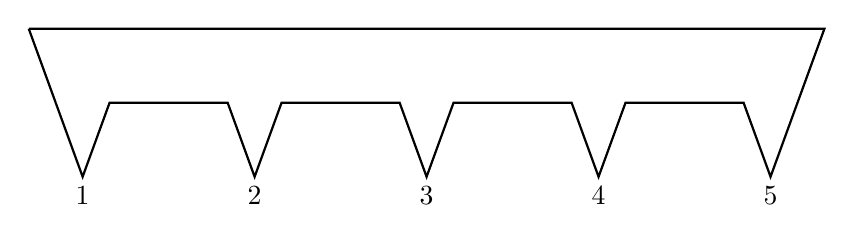
\begin{tikzpicture}[scale=1]
\coordinate (O) at (0,0);
\draw [thick] (O) -- (++110:1cm) coordinate (P);
\draw[thick] (O) --
  ++(-70:1cm) coordinate(A) node[below] {$1$} -- 
  ++(+70:1cm) -- ++(0:1.5cm) --
  ++(-70:1cm) coordinate(B) node[below] {$2$} -- 
  ++(+70:1cm) -- ++(0:1.5cm) --
  ++(-70:1cm) coordinate(C) node[below] {$3$}-- 
  ++(+70:1cm) -- ++(0:1.5cm) --
  ++(-70:1cm) coordinate(D) node[below] {$4$} -- 
  ++(+70:1cm) -- ++(0:1.5cm) --
  ++(-70:1cm) coordinate(E) node[below] {$5$} --
  ++(+70:2cm) -- (P);
\end{tikzpicture}
\selectlanguage{hebrew}
\caption{מוזיאון שקירותיו אינם יוצרים מצולע קמור}\label{f.museum.nonconvex}
\end{center}
\end{figure}

\begin{figure}[tb]
\begin{center}
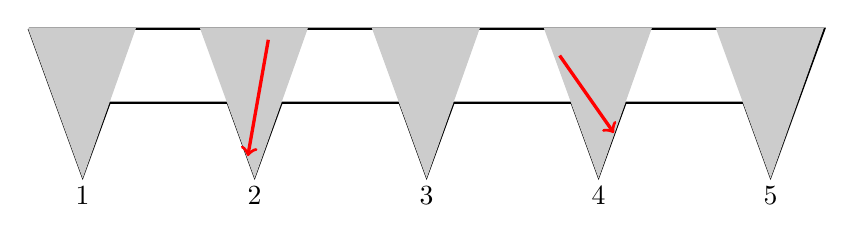
\begin{tikzpicture}[scale=1]
\coordinate (O) at (0,0);
\draw [thick] (O) -- (++110:1cm) coordinate (P);
\draw[thick] (O) --
  ++(-70:1cm) coordinate(A) node[below] {$1$} -- 
  ++(+70:1cm) -- ++(0:1.5cm) --
  ++(-70:1cm) coordinate(B) node[below] {$2$} -- 
  ++(+70:1cm) -- ++(0:1.5cm) --
  ++(-70:1cm) coordinate(C) node[below] {$3$}-- 
  ++(+70:1cm) -- ++(0:1.5cm) --
  ++(-70:1cm) coordinate(D) node[below] {$4$} -- 
  ++(+70:1cm) -- ++(0:1.5cm) --
  ++(-70:1cm) coordinate(E) node[below] {$5$} --
  ++(+70:2cm) -- (P);

\draw[fill,black!20!white] (A) -- ++(110:2cm) -- ++(0:1.35cm)-- cycle;
\draw[fill,black!20!white] (B) -- ++(110:2cm) -- ++(0:1.35cm)-- cycle;
\draw[fill,black!20!white] (C) -- ++(110:2cm) -- ++(0:1.35cm)-- cycle;
\draw[fill,black!20!white] (D) -- ++(110:2cm) -- ++(0:1.35cm)-- cycle;
\draw[fill,black!20!white] (E) -- ++(110:2cm) -- ++(0:1.35cm)-- cycle;

\draw[->,red,very thick] (2.7,.8) -- +(-100:1.5cm);
\draw[->,red,very thick] (6.4,.6) -- +(-55:1.2cm);
%\draw[->,very thick,green] (9,.9) -- (C);
%\draw[->,very thick,blue] ($(O)+(.5,.5)$) -- ++(7.5,.42);
%\draw[->,very thick,blue] ($(O)+(.5,.5)$) -- ++(3,-.5);
\end{tikzpicture}
\selectlanguage{hebrew}
\caption{נראות בתוך כל "שן"}\label{f.visibility-tooth}
\end{center}
\end{figure}

אם השומרת ניצבת בקירבת הקיר העליון, היא יכולה לראות את כל הקירות האופקיים (חיצים כחולים באיור%
~\ref{f.museum.shaded}).
מכאן שחמש שומרות מספיקות כדי לצפות על כל הקירות. בגלל שהמשולשים אינם נחתכים, שומרת במשולש אחד לא יכולה לראות את כל הקירות של משולש אחר (חץ ירוק) ולכן נחוצות חמש שומרות .
\begin{figure}[tb]
\begin{center}
\begin{tikzpicture}[scale=1]
\coordinate (O) at (0,0);
\draw [thick] (O) -- (++110:1cm) coordinate (P);
\draw[thick] (O) --
  ++(-70:1cm) coordinate(A) node[below] {$1$} -- 
  ++(+70:1cm) -- ++(0:1.5cm) --
  ++(-70:1cm) coordinate(B) node[below] {$2$} -- 
  ++(+70:1cm) -- ++(0:1.5cm) --
  ++(-70:1cm) coordinate(C) node[below] {$3$}-- 
  ++(+70:1cm) -- ++(0:1.5cm) --
  ++(-70:1cm) coordinate(D) node[below] {$4$} -- 
  ++(+70:1cm) -- ++(0:1.5cm) --
  ++(-70:1cm) coordinate(E) node[below] {$5$} --
  ++(+70:2cm) -- (P);

\draw[fill,black!20!white] (A) -- ++(110:2cm) -- ++(0:1.35cm)-- cycle;
\draw[fill,black!20!white] (B) -- ++(110:2cm) -- ++(0:1.35cm)-- cycle;
\draw[fill,black!20!white] (C) -- ++(110:2cm) -- ++(0:1.35cm)-- cycle;
\draw[fill,black!20!white] (D) -- ++(110:2cm) -- ++(0:1.35cm)-- cycle;
\draw[fill,black!20!white] (E) -- ++(110:2cm) -- ++(0:1.35cm)-- cycle;

%\draw[->,red,very thick] (2.7,1) -- (B);
\draw[->,very thick,green,dashed] (9,.8) -- +(-165:4.6cm);
\draw[->,very thick,blue] ($(O)+(.5,.5)$) -- ++(7.4,.4);
\draw[->,very thick,blue] ($(O)+(.5,.5)$) -- ++(2.9,-.45);
\draw (6,0) circle(4pt);
\draw (4.95,-.28) circle(4pt);
\end{tikzpicture}
\selectlanguage{hebrew}
\caption{נראות של קירות מוזיאון}\label{f.museum.shaded}
\end{center}
\end{figure}

ניתן להכליל את הדוגמה באיור%
~\ref{f.museum.nonconvex}
ולהראות שנחוצות
$n/3$
שומרות. המשך הפרק מוקדש להוכחה שמספיקות
$n/3$
שומרות לשמירה על כל מוזיאון.

סעיף%
~\ref{s.museum-triangulating}
מוכיח שניתן לצבוע כל מצולע מתולת
\L{(triangulated)}
בשלושה צבעים. נשתמש במשפט זה בסעיף%
~\ref{s.museum-guard}
כי להוכיח שמספיקות
$n/3$
שומרות. סעיף%
~\ref{s.museum-triangulated}
משלים את ההוכחה ומראה שניתן לתלת כל מצולע.

%%%%%%%%%%%%%%%%%%%%%%%%%%%%%%%%%%%%%%%%%%%%%%%%%%

\section{צביעת מצולעים מתולתים}\label{s.museum-triangulating}

\begin{definition}
\textbf{אלכסון \L{(diagonal)}}
של מצולע הוא קטע המחבר שני קודקודים והוא אינו אחת מהצלעות (החיצוניות) של המצולע.
\end{definition}
\begin{definition}
ניתן 
\textbf{לתלת}
\L{(triangulate)}
מצולע אם ניתן להעביר אלכסונים כך שהשטח הפנימי של המצולע מכוסה על ידי משולשים.
\end{definition}
\begin{theorem}\label{thm.tri}
ניתן לתלת כל מצולע.
\end{theorem}
אנו דוחים את ההוכחה של משפט%
~\ref{thm.tri}
לשלב מאוחר יותר.
\begin{definition}
קודקוד במצולע הוא 
\textbf{קמור}
אם הזווית הפנימית שלו קטנה מ-%
$180^\circ$.
קודקוד במצולע הוא
\textbf{קעור}
אם הזווית הפנימית שלו גדולה מ-%
$180^\circ$.

במצולע באיור%
~\ref{f.museum.arbitrary}
קודקוד 
$1$
קמור וקודקוד
$2$
קעור.
\end{definition}
\begin{figure}[tb]
\begin{center}
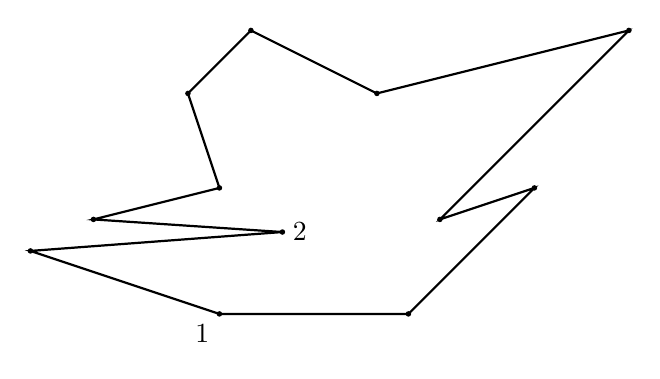
\begin{tikzpicture}[scale=.8]
\draw[thick]
  (0,0) coordinate (A) node[below left] {$1$} -- 
  ++(3,0) coordinate (B) --
  ++(2,2) coordinate (C) --
  ++(-1.5,-.5) coordinate (D) --
  ++(3,3) coordinate (E) -- 
  ++(-4,-1) coordinate (F) --
  ++(-2,1) coordinate (G) --
  ++(-1,-1) coordinate (H) --
  ++(.5,-1.5) coordinate (I) --
  ++(-2,-.5) coordinate (J) --
  ++(3,-.2) coordinate (K) node[right] {$2$} -- 
  ++(-4,-.3) coordinate (L) --
  cycle;
  
\foreach \point in {A,B,C,D,E,F,G,H,I,J,K,L}
  \fill (\point) circle(1.25pt);
\end{tikzpicture}
\end{center}
\selectlanguage{hebrew}
\caption{מצולע עם קודקוד קמור
($1$)
וקודקוד קעור
($2$)}\label{f.museum.arbitrary}
\end{figure}

\begin{definition}
ניתן
\textbf{לצבוע מצולע בשלושה צבעים}
אם קיימת העתקה:
\[
c: V \mapsto \{\textrm{\R{אדום, כחול, ירוק}}\},
\]
כך ששני הקודקודים של צלע מקבלים צבעים שונים.
\end{definition}
\begin{theorem}
ניתן לצבוע מצולע מתולת בשלושה צבעים.
\label{thm.colored}
\end{theorem}
\begin{proof}
באינדוקציה על מספר הקודקודים. ניתן לצבוע משולש בשלושה צבעים. למצולע עם 
$n>3$
קודקודים חייב להיות אלכסון. נבחר אלכסון שרירותי
$\overline{AB}$
(איור~%
\ref{f.museum.three-1})
ונחלק את המצולע לאורך האלכסון לשני מצולעים קטנים יותר
(איור~%
\ref{f.museum.three-2}).
לפי הנחת האינדוקציה ניתן לצבוע כל אחד מהמצולעים הללו בשלושה צבעים 
(איור~%
\ref{f.museum.three-3}).

\begin{figure}[tb]
\begin{center}
\begin{subfigure}{.4\textwidth}\centering
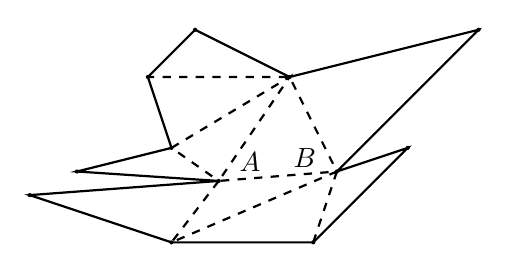
\begin{tikzpicture}[scale=.6]
\draw[thick]
  (0,0) coordinate (A) -- 
  ++(3,0) coordinate (B) --
  ++(2,2) coordinate (C) --
  ++(-1.5,-.5) coordinate (D) --
  ++(3,3) coordinate (E) -- 
  ++(-4,-1) coordinate (F) --
  ++(-2,1) coordinate (G) --
  ++(-1,-1) coordinate (H) --
  ++(.5,-1.5) coordinate (I) --
  ++(-2,-.5) coordinate (J) --
  ++(3,-.2) coordinate (K) -- 
  ++(-4,-.3) coordinate (L) --
  cycle;
  
\foreach \point in {A,B,C,D,E,F,G,H,I,J,K,L}
  \fill (\point) circle(1.25pt);

\node[above right,xshift=4pt] at (K) {$A$};
\node[above left,xshift=-4pt,yshift=-2pt] at (D) {$B$};

\draw[thick,dashed]
  (B) -- (D) -- (K) -- (F) -- (I) -- (K) -- (A) -- (D) -- (F) -- (H);
\end{tikzpicture}
\selectlanguage{hebrew}
\caption{אלכסון שרירותי במצולע}\label{f.museum.three-1}
\end{subfigure}
\hspace{3em}
\begin{subfigure}{.4\textwidth}\centering
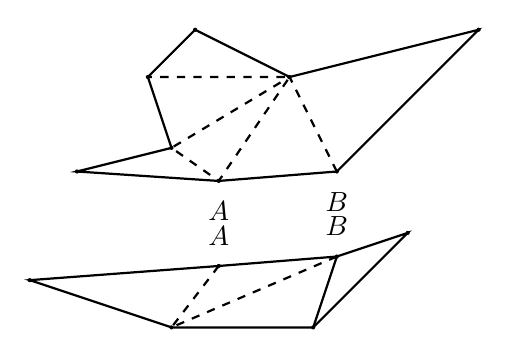
\begin{tikzpicture}[scale=.6]
\path
  (0,0) coordinate (A1) -- 
  ++(3,0) coordinate (B1) --
  ++(2,2) coordinate (C1) --
  ++(-1.5,-.5) coordinate (D1);
\draw[thick]
  (D1) --
  ++(3,3) coordinate (E1) -- 
  ++(-4,-1) coordinate (F1) --
  ++(-2,1) coordinate (G1) --
  ++(-1,-1) coordinate (H1) --
  ++(.5,-1.5) coordinate (I1) --
  ++(-2,-.5) coordinate (J1) --
  ++(3,-.2) coordinate (K1);
\path
  (K1) -- 
  ++(-4,-.3) coordinate (L1) --
  (A1);
  
\foreach \point in {D1,E1,F1,G1,H1,I1,J1,K1}
  \fill (\point) circle(1.25pt);

\node[below,yshift=-4pt] at (K1) {$A$};
\node[below,yshift=-4pt] at (D1) {$B$};

\draw[thick,dashed]
  (D1) -- (F1) -- (I1) -- (K1) -- (F1) -- (H1);
\draw[thick] (D1) -- (K1);

\begin{scope}[yshift=-1.8cm]

\draw[thick]
  (0,0) coordinate (A2) -- 
  ++(3,0) coordinate (B2) --
  ++(2,2) coordinate (C2) --
  ++(-1.5,-.5) coordinate (D2);
\path
  (D2) --
  ++(3,3) coordinate (E2) --
  ++(-4,-1) coordinate (F2) --
  ++(-2,1) coordinate (G2) --
  ++(-1,-1) coordinate (H2) --
  ++(.5,-1.5) coordinate (I2) --
  ++(-2,-.5) coordinate (J2) --
  ++(3,-.2) coordinate (K2);
\draw[thick]
  (K2) --
  ++(-4,-.3) coordinate (L2) --
  (A2);
  
\foreach \point in {A2,B2,C2,D2,K2,L2}
  \fill (\point) circle(1.25pt);
  
\node[above,yshift=4pt] at (K2) {$A$};
\node[above,yshift=4pt] at (D2) {$B$};

\draw[thick,dashed]
  (K2) -- (A2) -- (D2) -- (B2) -- (D2);
\draw[thick] (D2) -- (K2);

\end{scope}
\end{tikzpicture}
\selectlanguage{hebrew}
\caption{חלק את המצולע}\label{f.museum.three-2}
\end{subfigure}
\end{center}
\end{figure}

\begin{figure}[tb]
\begin{center}
\begin{subfigure}{.4\textwidth}\centering
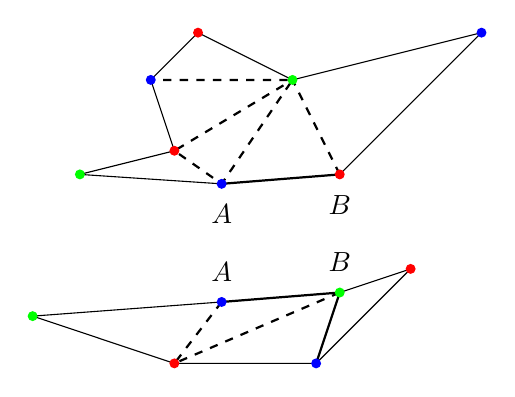
\begin{tikzpicture}[scale=.6]
\path
  (0,0) coordinate (A1) -- 
  ++(3,0) coordinate (B1) --
  ++(2,2) coordinate (C1) --
  ++(-1.5,-.5) coordinate (D1);
\draw
  (D1) --
  ++(3,3) coordinate (E1) -- 
  ++(-4,-1) coordinate (F1) --
  ++(-2,1) coordinate (G1) --
  ++(-1,-1) coordinate (H1) --
  ++(.5,-1.5) coordinate (I1) --
  ++(-2,-.5) coordinate (J1) --
  ++(3,-.2) coordinate (K1);
\path
  (K1) -- 
  ++(-4,-.3) coordinate (L1) --
  (A1);
  
\draw[thick,dashed]
  (D1) -- (F1) -- (I1) -- (K1) -- (F1) -- (H1);
\draw[thick] (D1) -- (K1);

\node[below,yshift=-4pt] at (K1) {$A$};
\node[below,yshift=-4pt] at (D1) {$B$};

\foreach \point/\color in {D1/red,E1/blue,F1/green,G1/red,H1/blue,I1/red,J1/green,K1/blue}
  \fill[color=\color] (\point) circle(3pt);

\begin{scope}[yshift=-2.5cm]

\draw
  (0,0) coordinate (A2) -- 
  ++(3,0) coordinate (B2) --
  ++(2,2) coordinate (C2) --
  ++(-1.5,-.5) coordinate (D2);
\path
  (D2) --
  ++(3,3) coordinate (E2) --
  ++(-4,-1) coordinate (F2) --
  ++(-2,1) coordinate (G2) --
  ++(-1,-1) coordinate (H2) --
  ++(.5,-1.5) coordinate (I2) --
  ++(-2,-.5) coordinate (J2) --
  ++(3,-.2) coordinate (K2);
\draw
  (K2) --
  ++(-4,-.3) coordinate (L2) --
  (A2);
  
\draw[thick,dashed]
  (K2) -- (A2) -- (D2) -- (B2) -- (D2);
\draw[thick] (D2) -- (K2);
\node[above,yshift=4pt] at (K2) {$A$};
\node[above,yshift=4pt] at (D2) {$B$};

\foreach \point/\color in {A2/red,B2/blue,C2/red,D2/green,K2/blue,L2/green}
  \fill[color=\color] (\point) circle(3pt);

\end{scope}
\end{tikzpicture}
\selectlanguage{hebrew}
\caption{צבע את שני המצולעים הקטנים בשלושה צבעים}\label{f.museum.three-3}
\end{subfigure}
\hspace{3em}
\begin{subfigure}{.4\textwidth}\centering
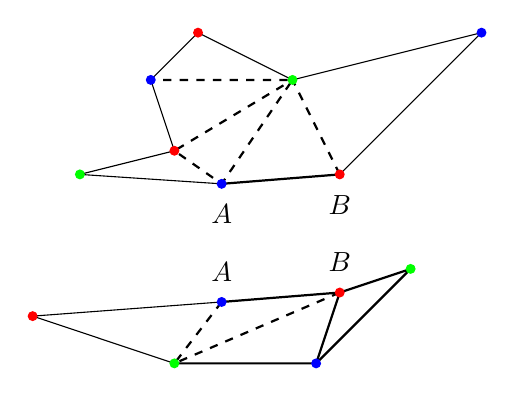
\begin{tikzpicture}[scale=.6]
\path
  (0,0) coordinate (A1) -- 
  ++(3,0) coordinate (B1) --
  ++(2,2) coordinate (C1) --
  ++(-1.5,-.5) coordinate (D1);
\draw
  (D1) --
  ++(3,3) coordinate (E1) -- 
  ++(-4,-1) coordinate (F1) --
  ++(-2,1) coordinate (G1) --
  ++(-1,-1) coordinate (H1) --
  ++(.5,-1.5) coordinate (I1) --
  ++(-2,-.5) coordinate (J1) --
  ++(3,-.2) coordinate (K1);
\path
  (K1) -- 
  ++(-4,-.3) coordinate (L1) --
  (A1);
  
\node[below,yshift=-4pt] at (K1) {$A$};
\node[below,yshift=-4pt] at (D1) {$B$};

\draw[thick,dashed]
  (D1) -- (F1) -- (I1) -- (K1) -- (F1) -- (H1);
\draw[thick] (D1) -- (K1);

\foreach \point/\color in {D1/red,E1/blue,F1/green,G1/red,H1/blue,I1/red,J1/green,K1/blue}
  \fill[color=\color] (\point) circle(3pt);

\begin{scope}[yshift=-2.5cm]

\draw[thick]
  (0,0) coordinate (A2) -- 
  ++(3,0) coordinate (B2) --
  ++(2,2) coordinate (C2) --
  ++(-1.5,-.5) coordinate (D2);
\path
  (D2) --
  ++(3,3) coordinate (E2) --
  ++(-4,-1) coordinate (F2) --
  ++(-2,1) coordinate (G2) --
  ++(-1,-1) coordinate (H2) --
  ++(.5,-1.5) coordinate (I2) --
  ++(-2,-.5) coordinate (J2) --
  ++(3,-.2) coordinate (K2);
\draw
  (K2) --
  ++(-4,-.3) coordinate (L2) --
  (A2);
  
\draw[thick,dashed]
  (K2) -- (A2) -- (D2) -- (B2) -- (D2);
\draw[thick] (D2) -- (K2);
\node[above,yshift=4pt] at (K2) {$A$};
\node[above,yshift=4pt] at (D2) {$B$};

\foreach \point/\color in {A2/green,B2/blue,C2/green,D2/red,K2/blue,L2/red}
  \fill[color=\color] (\point) circle(3pt);

\end{scope}
\end{tikzpicture}
\selectlanguage{hebrew}
\caption{החלף את הצבעים במצולע אחד כדי להתאים לשני}\label{f.museum.three-4}
\end{subfigure}
\end{center}
\end{figure}

ההעתקה של קודקודים לצבעים היא שרירותית, כך שאם הקודקודים 
$A,B$
מקבלים צבעים שונים בשני המצולעים, ניתן לשנות את הצבעים באחד מהם כך שהצבעים של 
$A,B$
זהים בשני המצולעים. למשל, נחליף את הצבעים
\textbf{אדום}
ו-%
\textbf{ירוק}
במצולע התחתון 
(איור%
~\ref{f.museum.three-3}).
נדביק את שני המצולעים כדי לשחזר את המצולע המקורי עם
$n$
קודקודים 
(איור%
~\ref{f.museum.three-4}).
המצולע יהיה צבוע בשלושה צבעים (איור%
~\ref{f.museum.three-5}). 
\end{proof}

\begin{figure}[tb]
\begin{center}
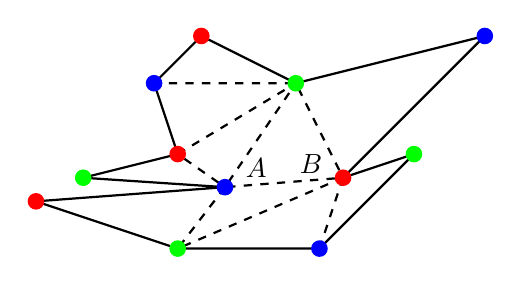
\begin{tikzpicture}[scale=.6]
\draw[thick]
  (0,0) coordinate (A) -- 
  ++(3,0) coordinate (B) --
  ++(2,2) coordinate (C) --
  ++(-1.5,-.5) coordinate (D) --
  ++(3,3) coordinate (E) -- 
  ++(-4,-1) coordinate (F) --
  ++(-2,1) coordinate (G) --
  ++(-1,-1) coordinate (H) --
  ++(.5,-1.5) coordinate (I) --
  ++(-2,-.5) coordinate (J) --
  ++(3,-.2) coordinate (K) -- 
  ++(-4,-.3) coordinate (L) --
  cycle;
  

\node[above right,xshift=4pt] at (K) {$A$};
\node[above left,xshift=-4pt,yshift=-2pt] at (D) {$B$};

\draw[thick,dashed]
  (B) -- (D) -- (K) -- (F) -- (I) -- (K) -- (A) -- (D) -- (F) -- (H);

\foreach \point/\color in {D/red,E/blue,F/green,G/red,H/blue,I/red,J/green,K/blue,A/green,B/blue,C/green,L/red}
  \fill[color=\color] (\point) circle(5pt);
\end{tikzpicture}
\end{center}
\selectlanguage{hebrew}
\caption{הדבק חזרה את שני המצולעים הקטנים}\label{f.museum.three-5}
\end{figure}

%%%%%%%%%%%%%%%%%%%%%%%%%%%%%%%%%%%%%%%%%%%%%%%%%%

\section{מצביעת מצולעים לשמירה על מוזיאונים}\label{s.museum-guard}

\begin{theorem}
$n/3$
שומרים יכולים לשמור על מוזיאון עם 
$n$
קירות.
\end{theorem}
\begin{proof}
לפי משפט
\ref{thm.tri}
ניתן לתלת את המצולע ולפי משפט
\ref{thm.colored}
ניתן לצבוע את המצולע בשלושה צבעים. שלושת הקודקודים של כל משולש יהיו צבועים בצבעים שונים כדי שכל צבע יופיע באחד הקודקודים של כל משולש. אם צובעים 
$n$
קודקודים בשלושה צבעים, צבע אחד לפחות, נניח אדום, יופיע לכל היותר
$n/3$
פעמים, ובכל משולש חייב להיות קודקוד צבוע אדום. נציב שומרת בכל קודקוד אדום, והיא יכולה לראות את הקירות של אותו משולש. כל המשולשים של תילות המצולע כוללים את כל צלעות המצולע, ולכן
$n/3$
שומרות מספיקות כדי לראות את כל קירות המוזיאון.
\end{proof}

אם
$n$
אינו מתחלק ב-%
$3$
מספר השומרות הדרוש הוא
$\lfloor n/3\rfloor$, 
המספר השלם הגדול ביותר שקטן או שווה ל-%
$n/3$.
למשל, 
$4$
שומרות מספיקות למוזיאון עם 
$12, 13, 14$
קירות, כי
$\lfloor 12/3\rfloor =\lfloor 13/3\rfloor=\lfloor 14/3\rfloor=4$. 
למען הפשטות נתעלם מסיבוך זה.

%%%%%%%%%%%%%%%%%%%%%%%%%%%%%%%%%%%%%%%%%%%%%%%%%%

\newpage

\section{ניתן לתלת כל מצולע}\label{s.museum-triangulated}

\begin{theorem}\label{thm.interior-angles-of-a-polygon}
סכום הזוויות הפנימיות של מצולע בעל
$n$
צלעות הוא
$180^\circ(n-2)$.
\end{theorem}

\begin{proof}
תחילה נוכיח עבור מצולעים קמורים. נסמן את 
\textbf{הזוויות החיצוניות}
ב-%
$\theta_i$
(איור%
~\ref{f.museum.exterior}).
אם נחבר את הזוויות החיצוניות נקבל:
\[ 
\displaystyle\sum_{i=1}^n \theta_i = 360^\circ\,.
\]
עבור כל זוית חיצונית
$\theta_i$
נסמן את הזוית הפנימית באותו קודקוד ב-%
$\phi_i$.
נחשב:
\begin{eqn}
\displaystyle\sum_1^n \theta_i &=&\displaystyle\sum_1^n (180^\circ-\phi_i)= 360^\circ\\
%n\cdot 180^\circ-\displaystyle\sum_1^n \phi_i &=& 360^\circ\\
\displaystyle\sum_1^n \phi_i &=& n\cdot 180^\circ-360^\circ =180^\circ(n-2)\,.
\end{eqn}
\begin{figure}[tb]
\begin{center}
\begin{tikzpicture}[scale=.6]
\coordinate (O) at (0,0);
%\fill (O) circle (2pt);
\foreach \x/\name/\n/\po in {0/a/A/right,.6/b/B/above,1.6/c/C/left,2.4/d/D/below left,3.9/e/E/below right} {
  \coordinate (\name) at ($(O)+(\x*72+18:3cm)$);
%  \fill (\name) circle (1.5pt);
%  \node[\po] at (\name) {$\n$};
%\draw[dashed] (O) -- (\name);
}
\draw[thick] (a) -- (b) -- (c) -- (d) --(e) -- cycle;

\draw[thick,dashed] (a) 
  node[above,xshift=-2pt,yshift=8pt] {$\theta_1$} -- 
  ($(a)!2!(b)$);
\draw[thick,dashed] (b)
  node[above left,xshift=-8pt,yshift=0pt] {$\theta_2$} -- 
  ($(b)!1.7!(c)$);
\draw[thick,dashed] (c) 
  node[below left,xshift=-4pt,yshift=-2pt] {$\theta_3$} -- 
  ($(c)!1.7!(d)$);
\draw[thick,dashed] (d)
  node[below right,xshift=0pt,yshift=-4pt] {$\theta_4$} -- 
  ($(d)!1.5!(e)$);
\draw[thick,dashed] (e)
  node[right,xshift=4pt,yshift=4pt] {$\theta_5$} -- 
  ($(e)!1.7!(a)$);

\end{tikzpicture}
\end{center}
\selectlanguage{hebrew}
\caption{הזוויות החיצוניות של מצולע קמור}\label{f.museum.exterior}
\end{figure}
אם יש קודקוד קעור
($B$
באיור%
~\ref{f.museum.concave}),
קיים משולש המורכב משתי הצלעות שנפגשות בקודקוד הקעור והצלע המסומנת בקו מקווקוו. נחבר את זוויות המשולש:
\begin{eqn}
(180^\circ - \alpha) + (360^\circ - \beta) + (180^\circ - \gamma) &=& 180^\circ\\
\alpha + \beta + \gamma &=& 3\cdot 180^\circ\,.
\end{eqn}
סכום הזוויות הפנימיות גדל ב-%
$\alpha+\beta+\gamma$
ומספר הקודקודים גדל בשלוש, ולכן השוויון במשפט נשמר:
\begin{eqn}
\displaystyle\sum_1^n \phi_i + (\alpha + \beta + \gamma) &=& 180^\circ(n-2)+3\cdot 180^\circ\\
&=& 180^\circ((n+3)-2)\,.
\end{eqn}
\end{proof}
\begin{figure}[tb]
\begin{center}
\begin{tikzpicture}
\draw[thick] (0,0) -- (3,0) coordinate (A) node[above left,yshift=8pt] {$\alpha$} -- ++(60:2) coordinate (B) node[above,yshift=8pt] {$\beta$} -- ++(-60:2) coordinate (C) node[above right,yshift=8pt] {$\gamma$}  -- ++(3,0);

\draw ($(A)+(-.4,0)$) arc(180:60:.4);
\draw ($(B)+(-60:.3)$) arc(-60:240:.3);
\draw ($(C)+(.4,0)$) arc(0:120:.4);

\draw[thick,dashed] (A) -- (C);
\end{tikzpicture}
\end{center}
\selectlanguage{hebrew}
\caption{קודקוד קעור}\label{f.museum.concave}
\end{figure}
\begin{theorem}\label{thm.convex}
חייבים להיות לפחות שלושה קודקודים קמורים במצולע.
\end{theorem}
\begin{proof}
יהי
$k$
מספר הקודקודים הקעורים כאשר הזווית הפנימית של כל קודקוד היא
$180^\circ+\epsilon_i$, $\epsilon_i>0$.
סכום הזוויות הפנימיות של הקודקודים
\textbf{הקעורים}
הוא בוודאי קטן או שווה לסכום
\textbf{כל}
הזוויות הפנימיות:
\begin{eqn}
k\cdot 180^\circ +\displaystyle\sum_{i=1}^{k}\epsilon_i &\leq& 180^\circ(n-2)\\
k\cdot 180^\circ  &<& 180^\circ(n-2)\\
%(k+2)\cdot 180^\circ &<& n\cdot 180^\circ\\
k&<&n-2\,.
\end{eqn}
מכאן שיש לא רק קודקוד אחד אלא לפחות שלושה קודקודים שאינם קעורים.
\end{proof}

\begin{proof} \textbf{%
(משפט%
~\ref{thm.tri}
שניתן לתלת כל מצולע)}
באינדוקציה על מספר הקודקודים. עבור
$n=3$
אין מה להוכיח. נניח ש-%
$n>3$.
לפי משפט%
~\ref{thm.convex}
חייב להיות קודקוד קמור
$C$.
נסמן את הקודקודים השכנים שלו
$B,D$.
אם
$\overline{BD}$
נמצא כולו בתוך המצולע 
(איור~%
\ref{f.contained}),
אז הוא אלכסון וניתן לחלק את המצולע למשולש 
$\triangle BCD$
ולמצולע אחר
$\overline{ABDE}$
עם צלע
$\overline{BD}$.
לפי הנחת האינדוקציה ניתן לתלת את המצולע ואז להדביק אותו למשולש
$\triangle BCD$
ולקבל תילות של המצולע המקורי.
\begin{figure}[tb]
\begin{center}
\begin{subfigure}{.4\textwidth}\centering
\begin{tikzpicture}[scale=1.4]
\clip (-.5,-.4) rectangle (3.8,2.2);
\draw
  (0,0) coordinate (A) -- 
  ++(1.5,0) coordinate (B) --
  ++(2,2) coordinate (C) --
  ++(-1.8,-.5) coordinate (D) --
  ++(-1,.5) coordinate (E) --
  (A);
\draw[thick,dashed] (B) -- (D);
\foreach \point/\pos in {A/below,B/below,C/right,D/above,E/left}
  \node[\pos] at (\point) {$\point$};
\vertex{B};
\vertex{D};
\end{tikzpicture}
\selectlanguage{hebrew}
\caption{תילות כאשר האלכסון נמצא בתוך המצולע}\label{f.contained}
\end{subfigure}
\hspace{3em}
\begin{subfigure}{.4\textwidth}\centering
\begin{tikzpicture}[scale=1.4]
\clip (-.2,-.4) rectangle (3.8,2.2);
\draw
  (0,0) coordinate (A) -- 
  ++(1.5,0) coordinate (B) --
  ++(2,2) coordinate (C) --
  ++(-1.8,-.5) coordinate (D) --
  ++(-1,.5) coordinate (E) --
  ++(1.3,-1) coordinate (F) --
  (A);
\draw[thick,dashed] (B) -- (D);
\draw[very thick,dotted] (C) -- (F);
\node [draw,circle through=(F)] at (C) {};
\node[below] at (A) {$A$};
\node[below] at (B) {$B$};
\node[right] at (C) {$C$};
\node[above,yshift=2pt,xshift=-3pt] at (D) {$D$};
\node[left]  at (E) {$E$};
\node[below,yshift=-1pt,xshift=-2pt] at (F) {$F$};
\vertex{C};
\vertex{F};
\end{tikzpicture}
\selectlanguage{hebrew}
\caption{תילות כאשר האלכסון אינו בתוך המצולע}\label{f.museum.concave-vertices}
\end{subfigure}
\end{center}
\end{figure}

אם 
$\overline{BD}$
אינו בתוך המצולע, חייב להיות קודקוד קעור
$F$
הקרוב ביותר ל-%
$C$
(איור~%
\ref{f.museum.concave-vertices}).
$\overline{CF}$
הוא אלכסון המחלק את המצולע לשני מצולעים קטנים יותר
$\overline{CFED}$
ו-%
$\overline{CFAB}$.
לפי הנחת האינדוקציה ניתן לתלת אותם ולהדביק אותם זה לזה.
\end{proof}

%%%%%%%%%%%%%%%%%%%%%%%%%%%%%%%%%%%%%%%%%%

\subsection*{מה ההפתעה?}
משפט המוזיאון מפתיע כי ההוכחה של מה שנראה כמשפט בגיאומטריה משתמשת בצורה אלגנטית בצביעת גרפים.

\subsection*{מקורות}

פרק זה מבוסס על פרק~39 ב-%
\cite{thebook}.
